%Chapter 6: Conclusions

\chapter{Conclusions and Future Outlook}

The unifying theme throughout this dissertation has been that the optimal combination of geophysical data sets provides faster and more robust images of the seismic source and that this in turn can be used for hazards mitigation.

In Chapter 2 with data from the $M_w$7.2 April 4, 2010 El Mayor-Cucapah earthquake in northern Baja California we convincingly demonstrated that regional high-rate real-time GPS networks can become an essential tool for early warning and rapid earthquake response. We took this one step further by applying a Kalman filter to obtain an optimal combination of data from collocated high-rate GPS and very-high-rate accelerometer stations, which takes advantage of the strengths and minimizes the weaknesses of both data types. The result is a new methodology for providing displacement time series with millimeter precision which can be used to better characterize the seismic source. It provides an improved broadband record of ground displacements and velocities over the full range of frequencies sampled by the accelerometer data, as well as the static deformation. This approach is capable of precisely detecting P-wave arrivals of medium to large near-source earthquakes with dense networks of collocated GPS and seismic instruments, making it particularly valuable for earthquake early warning systems and rapid earthquake response. It also provides a powerful new analysis tool to study the rupture characteristics of large earthquakes. These results have been published in \citet{bock2011} and it's applications to early warning magnitude scaling have been published in \citet{Crowell2013}.

We also showed that automatic baseline correction schemes from accelerometer data alone can, for selected stations, provide useful strong motion (dynamic) displacements information. However, the static offsets determined by such automated schemes are often unreliable. Furthermore, adding a static field constraint to the baseline correction procedure does not guarantee convergence to the correct value and even if the correct static offset is obtained; other parts of the waveform might be in error by large amounts. The objective estimation of baseline-corrected displacements, even when incorporating reliable and independent information such as the static field estimated from GPS remains elusive. We have demonstrated that such a scheme, which eliminates the need for subjective judgment, is still fraught with problems. We tested the assumption that baseline corrections introduce errors only at long periods outside what is of engineering interest and find it does not hold for the 2011 Tohoku-oki data set. Analysis of the power spectral densities and displacement response spectra demonstrate that the frequency domain error incurred by the baseline correction is well within the frequency range of interest to both seismology and engineering. The Kalman filter method, which combines high rate GPS and accelerometer data, is not affected by these problems. We demonstrated that even for K-net accelerometer data set which displays behavior associated with large baseline offsets the Kalman filter solution routinely produces reliable broadband displacements. These results have been published in \citet{melgar2013robust}

In Chapter 3 we discussed the issue of rapid modeling of the earthquake source with static field data. We presented an approach for real-time computation of centroid moment tensors for large events from local and regional GPS displacement records. We used the coseismic offsets and Green�s functions for a layered Earth to relate the deformation at the surface with source parameters at depth. We demonstrated the algorithm with two test cases, the 2010 $M_w$ 7.2 El Mayor-Cucapah earthquake and the 2003 $M_w$ 8.3 Tokachi-oki earthquake. In both cases we have shown that provided with low latency access to displacement data it is feasible to obtain a robust centroid location and moment tensor solution within the first 2-3 minutes after rupture initiation. The algorithm is computationally efficient and thus amenable for rapid modeling and early detection. These results were published in \citet{melgar2012}

Also in Chapter 3 we discussed the application of the CMT methodology as a starting point for a static slip inversion of the 2011 $M_w$ 9 Tohoku-oki event. Considering the review of the sequence of events at the USGS National Earthquake Information Center (NEIC) \citep{hayes2011}, there are several stages where the independent information provided by the seismogeodetic time series could have been helpful for a great event such as Tohoku-oki. Both the NEIC and the Pacific Tsunami Warning Center obtained preliminary teleseismic $P$ wave locations and mechanisms within 5 minutes of the origin time, but the first public release was delayed until 9.7 minutes. Independent confirmation of the source size would provide confidence for releasing information earlier. The first two versions of ShakeMap and PAGER alerts were released with the affected areas based on point sources. The ShakeMap and Pager alerts were updated to a finite fault source, significantly extending the length of affected coastline after 2 hours and 42 minutes. Within 57 seconds after origin time the result of the line source \textit{fast}CMT and slip inversion solutions reproduced the main features of the rupture, approximately 340 km long with average slip of 15 m over the main source region. Additionally the \textit{fast}CMT solution has the correct fault orientation of 204$^\circ$ as opposed to 230$^\circ$ for the rapid finite fault inversion based on the W phase fault orientation. Early access to this information could provide confidence for earlier release of the finite fault corrected Global ShakeMap. Full integration and combination of GPS into seismic monitoring is essential for a hazard system that is more robust than either traditional seismic or geodetic monitoring alone. Because the \textit{fast}CMT algorithm does not require assumptions about the fault geometry, it is also applicable to source regions outside subduction zones. The ability to produce seismogeodetic displacement and velocity time series in real time implies that the delay for calculating near-real-time kinematic rupture models can also be significantly reduced. These results were published in \citet{melgar2013rapid}.

In Chapter 4 we further elaborated on the kinematic problem. We showed that the seismogeodetic data can be easily employed to obtain a time dependent rupture model of the 2011 Tohoku-oki source. Inversion of 3-component seismogeodetic data for 20 stations revealed features of the source which largely agree with teleseismic inversions and back projection results. We demonstrated that inclusion of the velocity time series produced by the seismogeodetic solution sharpens the picture of the source. We relied on Akaike's Bayesian information criterion formalism for determining optimal smoothing, thus largely removing the human element from the decision-making for the inversion parameters. The seimogeodetic kinematic inversion could potentially be available within minutes of rupture initiation of a large event. We also showed that rupture models from the seimogeodetic data can provide insights into the source process. We observe a heterogeneous rupture for the 2011 Tohoku-oki event, with marked differences between the up dip and down dip rupture behaviors. Very slow initial rupture is followed by fast up-dip rupture that expands quickly along-strike once rupture reaches the trench. Down dip we observe two distinct pulses of moment release with the later pulse possibly driven by the long duration of slip up-dip. Our results are in agreement with observations from low frequency back projection \citep{yagi2012} as well s broadband tele-seismic inversions \citep{shao2011}. We also showed that the model captures depth-dependent behavior of rupture. Frequency domain analysis of the source spectra shows that shallow subfaults are depleted in high frequency radiation with deeper subfaults being progressively enriched in short period energy. This agrees with the observations of \citet{kurahashi2011} who found that strong motions originated down-dip from the hypocenter as well as with the conceptual model of \citep{lay2012} who proposed that such depth-dependent observations are a consequences of changing frictional properties at depth.

In Chapter 5 we discussed the addition of offshore data in the form of tide gauges, real-time kinematic GPS buoys and ocean bottom pressure sensors into the source inversion process. First we show with the example of the 2011 Tohoku-oki earthquake a source modeling approach that relies on joint inversion of land-based estimates of coseismic deformation from collocated GPS/accelerometer stations and ocean-based wave gauges. We showed that the earthquake sources thus determined can be used as initial conditions to model tsunami propagation in the near-source coastline. We compared the results of such models against post-event survey data and concluded that the inundation forecasts could be used for tsunami early warning. We deduced that off-shore wave gauges in water shallower than previously thought (100-1000m) can be useful for tsunami forecast. However we found that coastal tide gauges are of limited use for the event studied. We argued that in the future joint inversion of these near source geophysical data and deployment of further ocean-based instruments can help to deliver timely and accurate early warning in regions of tsunami hazard. These results were published in \citet{melgar2013near}
 
We also showed in Chapter 5 the effect of adding the off-shore data into the kinematic modeling process and produce a time dependent model of the source that relies on both the land- and ocean-based observables. The tsunami data increases the level of complexity in the shallow portion of the fault model, it also increases the amplitude and duration of moment release in the shallow subfaults while leaving the deeper part of the model largely unchanged. The net-effect of the tsunami data is to increase the complexity of the shallowest portion of the fault model; it also produces significantly longer duration source time functions than the land-only kinematic inversion in the shallow sub-faults. We discussed the robustness of these features and argued that there are secondary sources of tsunami energy that might not be accounted for. Finally, we showed the differences between employing the time-varying deformation of bathymetry versus instantaneous deformation of the sea-floor as well as the effect of considering the tsunamigenic contributions of horizontal advection of sloping bathymetry. We argued that for near-field propagation simulations these two often ignored effects can be significant.

It is clear that employing more diverse geophysical data for modeling the earthquake source will aid in developing a more comprehensive image of the underlying processes. This stands to impact both our understanding of  large ruptures and our capability to respond to them rapidly. The ocean bottom stands to be the next frontier of seismological and geodetic exploration as technological improvements produce more and better instruments capable of measuring geophysical signals on the sea floor. Sea-floor geodesy has made significant advances \citep{burgmann2013} and technological developments such as wave gliders promise to make observations of sea-floor deformation denser and more widespread in the future. There exists also many deployments of ocean bottom seismic networks. These typically consist of high-gain broadband seismometers that cannot be used to study the rupture process of large events up close. Deployments of ocean-bottom strong motion sensors are few and far between. Nonetheless it is possible to repurpose already existing ocean bottom infrastructure to study large ruptures. For example most broadband ocean bottom seismometer deployments include pressure gauges. It has been known for some time that at long periods \citep{webb1998} bottom pressure fluctuations are proportional to vertical acceleration. 

Consider Figure \ref{fig_clay} where we have plotted the time series of a rare occurrence of an ocean bottom strong motion sensor and a collocated pressure gauge for the Clayoquot Slope station located 100km from the 2014 $M_w$6.5 event offshore Vancouver Island. At long periods (longer than 10s in this example) we can assume full water column response to the bottom accelerations (Figure \ref{fig_clay}a) \citep{filloux1983,webb1998,mofjeld2001}. We can convert between pressure and acceleration because the pressure recording (Figure \ref{fig_clay}b) will be proportional and in phase to the vertical acceleration. You can see from the 10s low-pass filtered comparisons in Figure \ref{fig_clay}c that the vertical accelerations predicted by the bottom pressure recording match the strong motions sensor well. The Clayoquot Slope station is an exception, rather than the norm, since strong motion sensors are seldom found at ocean bottom sites. Pressure sensors however are widespread. In fact DART buoys (which rely on absolute pressure gauges) routinely record seismic waves \citep{mofjeld2001}. Figure \ref{fig_dart} shows an example of two DART buoys the day of the $M_w$ 6.8 Ferndale event offshore Northern California. Both buoys record transient sea-surface height changes of up to 20cm peak-to-peak, but no tsunami follows. This is because the Ferndale event was a strike slip earthquake with no appreciable vertical deformation of the sea floor. In fact the timing of the arrivals at the DART buoys coincides with the Rayleigh waves. The bottom pressure sensor of the buoys incorrectly identifies the vertical accelerations as actual changes of the sea surface height. These observations suggest that it is possible that dense networks of ocean bottom strong motion sensors, in the form of pressure gauges, already exist. An exciting avenue of research will be how to incorporate these, and other ocean bottom sensing techniques into the study of large earthquakes.

\begin{figure}[!ht] 
  \centering
  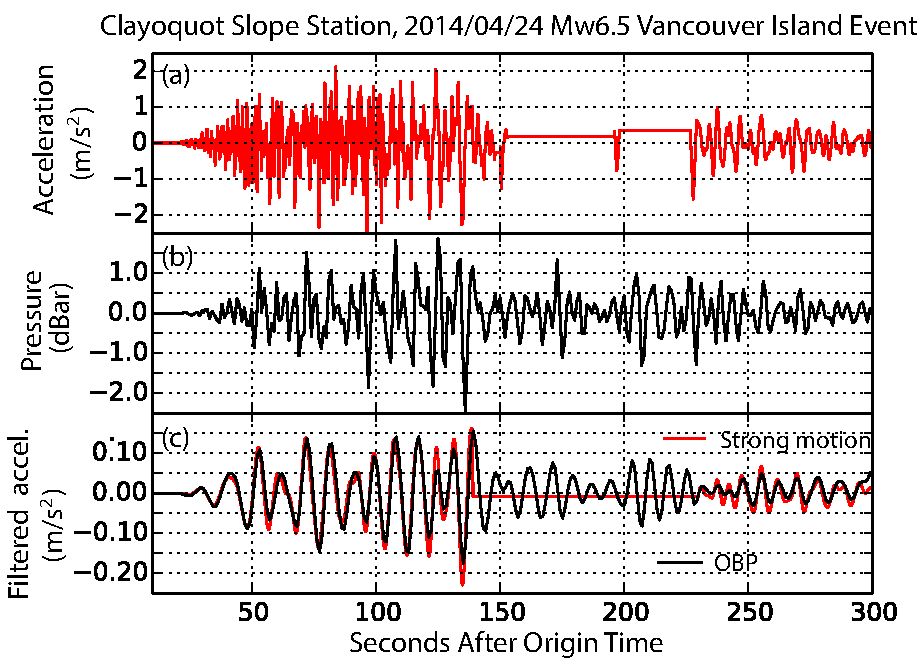
\includegraphics[width=0.9\linewidth]{./figures/ch6/timeseries.pdf}
    \caption[Ocean bottom strong motion recording for the $M_w$6.5 2014 Vancouver Island event]{Ocean bottom strong motion recording for the $M_w$6.5 2014 Vancouver Island event. (a) is the raw vertical strong motion accelerogram, (b) is the raw pressure recording and (c) is the 10s low pass filtered accelerogram and predicted acceleration from the pressure gauge. The flat segments in the accelerometer time series are gaps in the data}
  \label{fig_clay}
\end{figure}

\begin{figure}[!ht] 
  \centering
  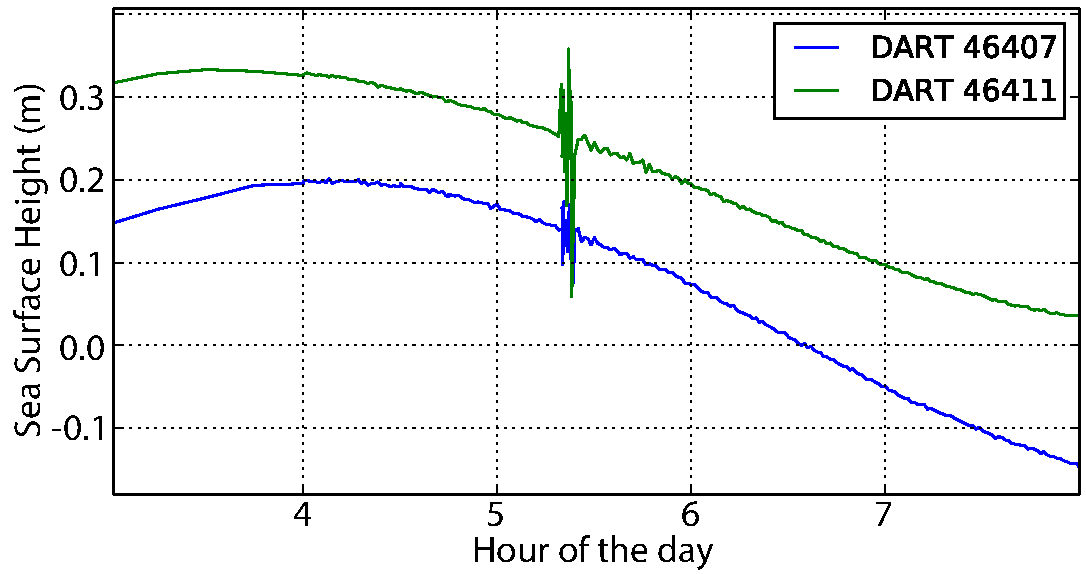
\includegraphics[width=0.9\linewidth]{./figures/ch6/DART.pdf}
    \caption[DART buoy recordings following the $M_w$ 6.8 Ferndale strike slip event off-shore Northern California]{DART buoy recordings following the $M_w$ 6.8 Ferndale strike slip event off-shore Northern California}
  \label{fig_dart}
\end{figure}

A similar situation exists for tsunami observations. High quality pressure gauges such as DART buoys and the cabled observatories used in Chapters 4 and 5 offshore Japan are sparse. Seldom do we have dense observations of tsunami propagation. The differential pressure gauges often deployed with high-gain OBS deployments can offer a unique opportunity to study tsunami physics. Figure \ref{fig_kuril} shows the differential pressure gauge recordings for 26 stations around the Hawaii islands deployed as part of the PLUME project \citep{wolfe2009}.  Comparatively dense observations such as these can elucidate details on the propagation characteristics of tsunamis. Local bathymetry plays a major role in tsunami intensity \citep{wang2007,iglesias2014}, akin to site amplification due to local geology in seismology. Understanding these effects is important to quantifying local hazards both from tele-tsunamis and regional ones. Indeed there is significant heterogeneity in the recordings shown in Figure \ref{fig_kuril}.

\begin{figure}[!ht] 
  \centering
  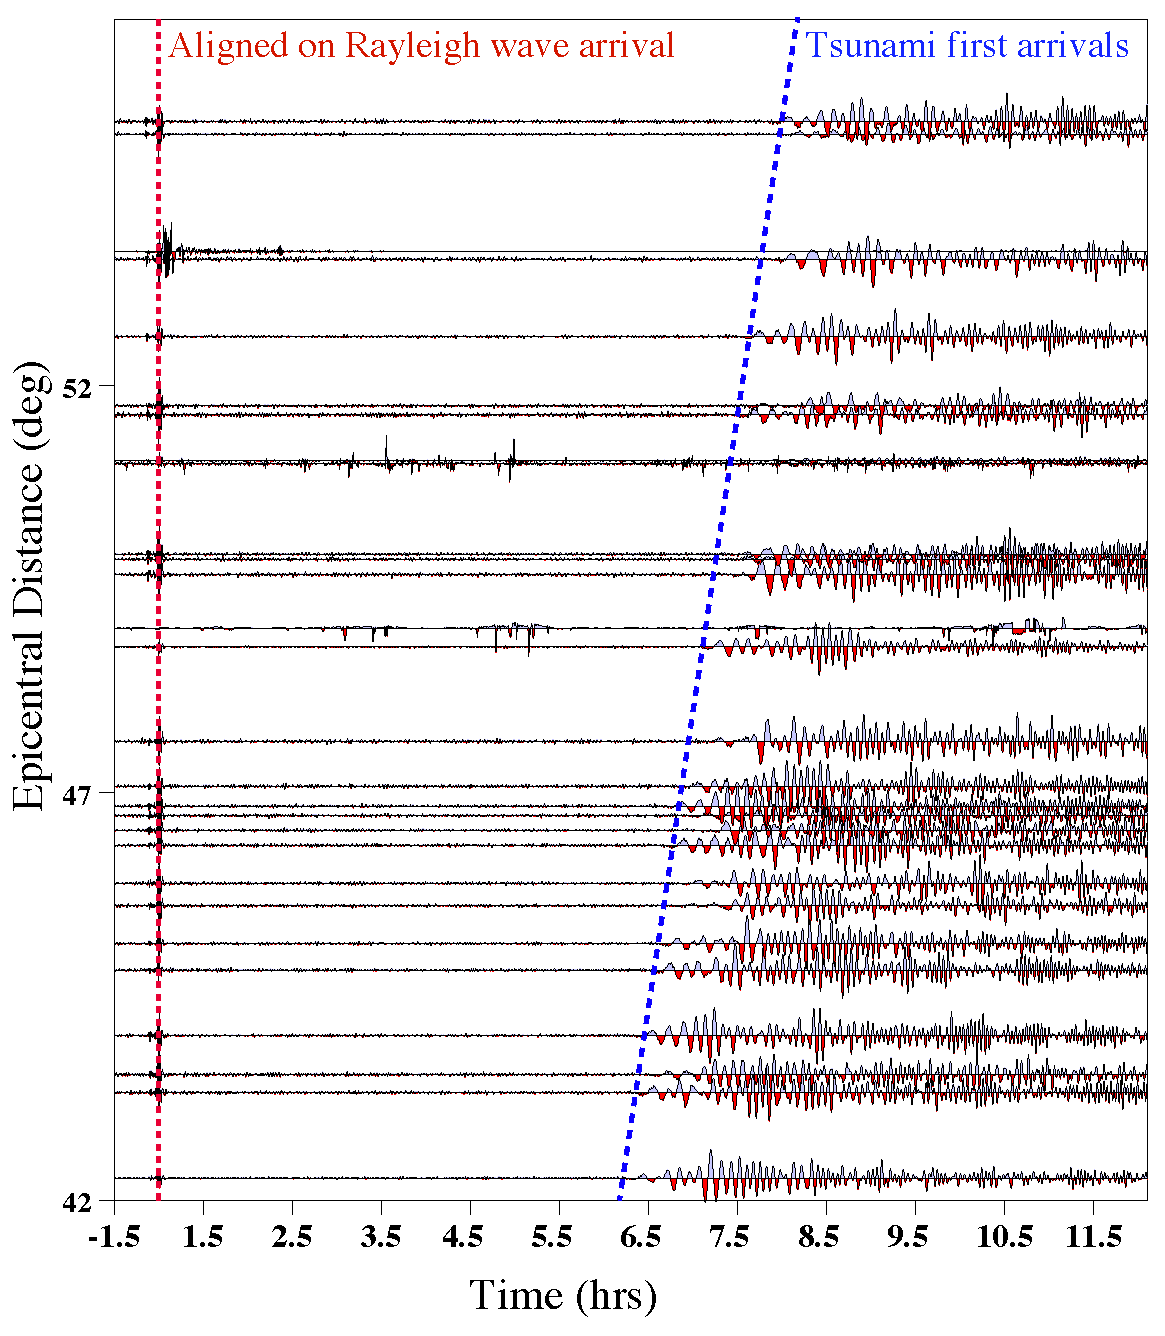
\includegraphics[width=0.8\linewidth]{./figures/ch6/kdpg-dist.pdf}
    \caption[Differential pressure gauge recordings at 26 ocean bottom stations during the 2006 Kuril Islands tsunami]{Differential pressure gauge recordings at 26 ocean bottom stations during the 2006 Kuril Islands tsunami. The waveforms are aligned on the Rayleigh wave arrivals (red dotted line). The tsunami first arrivals are indicated by the blue dotted line.}
  \label{fig_kuril}
\end{figure}

Typically, tsunami and seismic waves have been considered parts of different disciplines, in reality, they are part of the same wavefield and it makes sense to study them jointly. The intersection of these two wavefields can provide new insights into source physics \citep{kozdon2014} and perhaps even new avenues to improve early warning and rapid response algorithms \citep{lotto2013}. With the simple examples of Figures \ref{fig_clay}-\ref{fig_kuril}  we have shown that there is already infrastructure in place to further this avenue of research and in the future we expect significant developments from joint geophysical observations such as these.

\FloatBarrier

\section{Acknowledgments}

The contents of this chapter are unpublished. We'd like to thank Ocean Networks Canada for the data for the Clayoquot Canyon station and the National Oceanographic and Atmospheric Administration for the DART buoy data. We would also like to thank Gabi Laske for providing the differential pressure gauge data for the PLUME project.
